%%%%%%%%%%%%%%%%%%%%%%%%%%%%%%%%%%%%%%%%%%%%%%%%%%%%%%%%%%%%%%%%%%%%%%%%%%%%%%%%
%2345678901234567890123456789012345678901234567890123456789012345678901234567890
%        1         2         3         4         5         6         7         8

\documentclass[letterpaper, 10 pt, conference]{ieeeconf}  % Comment this line out if you need a4paper

%\documentclass[a4paper, 10pt, conference]{ieeeconf}      % Use this line for a4 paper

\IEEEoverridecommandlockouts                              % This command is only needed if 
                                                          % you want to use the \thanks command

\overrideIEEEmargins                                      % Needed to meet printer requirements.

% See the \addtolength command later in the file to balance the column lengths
% on the last page of the document

% The following packages can be found on http:\\www.ctan.org
%\usepackage{graphics} % for pdf, bitmapped graphics files
%\usepackage{epsfig} % for postscript graphics files
%\usepackage{mathptmx} % assumes new font selection scheme installed
%\usepackage{times} % assumes new font selection scheme installed
%\usepackage{amsmath} % assumes amsmath package installed
%\usepackage{amssymb}  % assumes amsmath package installed

\title{\LARGE \bf
Learning to Learn in the Context of Spiking Neural Networks
}


\author{Moritz Zanger$^{1}$ % <-this % stops a space
\thanks{*This work was not supported by any organization}% <-this % stops a space
\thanks{$^{1}$Moritz Zanger, Faculty of Mechanical Engineering, Karlsruhe Institute of Technology
        {\tt\small zanger.moritz@googlemail.com}}%
}

\usepackage{graphicx}
\graphicspath{{./images/}}

\begin{document}

\maketitle
\thispagestyle{empty}
\pagestyle{empty}


%%%%%%%%%%%%%%%%%%%%%%%%%%%%%%%%%%%%%%%%%%%%%%%%%%%%%%%%%%%%%%%%%%%%%%%%%%%%%%%%
\begin{abstract}

L2L abstract - I will write it in the end

\end{abstract}


%%%%%%%%%%%%%%%%%%%%%%%%%%%%%%%%%%%%%%%%%%%%%%%%%%%%%%%%%%%%%%%%%%%%%%%%%%%%%%%%
\section{INTRODUCTION}

Introduction to the topic

\section{RECURRENT NEURAL NETWORKS}

\subsection{Subheading}

\subsection{Subheading2}

\section{SPIKING NEURAL NETWORKS (SNN)}

Second generation neural networks, as commonly described in the literature, base their neurons activation on various continuous functions 
and allow a larger space of operations. Maass et al. (Maass et al.) introduced a third setup for 
designing neural network models. This setup is based on a neuron model that integrates a different conception on how neurons are activated,
thus allowing a more accurate representation of biological neurons and their inner workings. This model of Spiking Neural Networks (SNN) employs
integrate-and-fire neurons (Maass et al.) which allow timing of activation pulses and therefore a potentially higher capability of representing 
information. 

\subsection{Neurons - Activation and Signal Processing} 

The process of signal transportation within biological neurons ...(figures and Gruning and Bohte)\newline

The fundemantal idea behind the computational units of an SNN revolves around integrating a temporal factor 
in the representation of information. Various models of these spiking neurons, such as the integrate-and-fire model (Abbott), 
the Hodgkin-Huxley model (Hodgkin and Huxley), the model by Izhikevich (Izhikevich) and the Spike Response Model by Gerstner (Gerstner) 
exist and vary in their attempt to trade off biological accuracy and computational complexity (Grunte and Bohte).
The Leaky-Integrate-and-Fire model is nowadays the most widespread apporach due to its simplicity and computational advantages. 
The representation of the activation process of the neron is modeled by an electrical circuit in which the membrane potential, threshold voltage,
resting potential and leak rate are realized through a capacitor, gate, battery and resistance respectively. (Abbott and fig. Ponulak)
\newline
At any moment, an LIF neuron has a drive v, which depends on its bias
current, b; its inputs a(in)j (where the index j runs from 1 to the number
of inputs); and its synaptic weights, Wj (Eliasmith and Anderson, 2002). (... and so on)

\subsection{Spike-based Neural Codes}

Whilst encoding and decoding of the desired information is much simpler and intuitive in second generation neural network models,
this is a larger challenge for the time-dependent neurons in an SNN, as there is an arbitrary 
number of theorically possible ways of encoding information in the neurons. In fact the biological process of information decoding is 
still being researched, whereas various methods have been introduced Neuroscience Enginering.

\begin{itemize}

        \item Rate Coding is an approach aiming at recording spike rates during fixed time frames. This implementation of spike encoding can be seen as an analog way of interpreting spike trains in SNNs.
        \item Latency Coding encodes spikes based on their timing rather than their multiplicity. This encoding has for example been used in unsupervised learning [43], and
        supervised learning methods like SpikeProp (S. Bohte, J. Kok)
        \item Fully temporal codes are a more general term which includes the above mentioned approaches. It encodes information based on the precise
        timing of each spike in a spike train. (Gruning and Bohte)
        \item Gaussian Coding applies a gaussian distribution over recorded spikes of each neuron and encodes information based on their stochastic occurence.
        \item ...
        
\end{itemize}        

\subsection{Learning in Spiking Neural Networks - Synaptic Plasiticity}

Whilst conventional neural networks employ a stochastic version of gradient descend to backpropagate erros throughout the network, the same approach
is difficult to apply in the realm of SNNs due to their temporal dependance and the non-differentiability of spike trains. Whereas multiple learning
rules adressing SNNs exist (such as Hebbian Rule, Binarization of ANNs, Conversion from ANNs and Variations of backpropagation (Pfeiffer and Pfeil)), a more 
biologically realistic training rule is introduced with the spike-timing-dependant plasiticy (STDP). The key feature of this approach is 
to adjust weights between a pre- and post-synaptic neuron according to their relative spike times within an interval of roughly tens of 
milliseconds in length (S. Bohte, J. Kok)
... more on STDP 

\subsubsection{Backpropagation and Feedback-alignment}


\subsubsection{Error Feedback}

\subsection{Performance of SNNs)}

\section{LEARNING TO LEARN (L2L)}

The field of reinforcement learning (RL) has recently celebrated great success at reaching human-like and even surpassing human abilities on
complex environments such as Atari and Go (Mnih et al. and Silver et al.) with the implementation of Deep Neural Networks to 
account for non-linear function approximation over high-dimensional action and state spaces. However Artificial Intelligence in general 
(Landsell and Kording) and Reinforcement Learning in particular (Dual et al.) currently suffer from two major drawbacks, 
that are limiting their application and design (J. Wang et al.): 
\begin{itemize}
        \item Firstly the immense volume of required training data and the relatively expensive generation of this data in often simulated
        environments.
        \item Secondly RL-algorithms often have to be heavily tailored to a specific range of tasks and various algorithms, each of which
        depending on numerous hyperparameters and thus requiring immense efforts compared to currently reached results.
\end{itemize}        

Botvinick et al. explain these weak spots in AI with a need for low learning rates and the bias-variance trade-off.
Low learning rates are necessary to prevent both catastrophic interference (discarding previously reached successful
configurations) and overfitting (Hardt, M. et al.). The bias-variance trade-off is a phenomenon describing the contrary 
working directions of efficiency-driving biases or priors and performing on a wider range of tasks. \newline

--------- maybe more basics from hochreiter et al. -------- \newline

With some approaches addressing these issues existing, Landsell and Kording argue, that these L2L approaches can be categorized into 
either Learning to Optimize or Structure Learning (Landsell and Kording). Learning to Optimize focusses on the general 
adaption of network parameters to achieve efficient learning rules on arbirary Task classes without hand-selection. Similiarly to the way
gradient descent applies small changes of the weights in an NN in order to minimize loss functions, the design of AI systems can be viewed as
an optimization problem itself, that requires parameter optimization to ensure a well performing algorithm. Structure Learning 
on the other hand makes use of structural similarities within a finite family of tasks to reach higher data
efficiency due to its prior adaptnedness to the given family of tasks(Landsell and Kording). \newline

\begin{figure}[thpb]
        \centering
        \framebox{\parbox{3in}{
        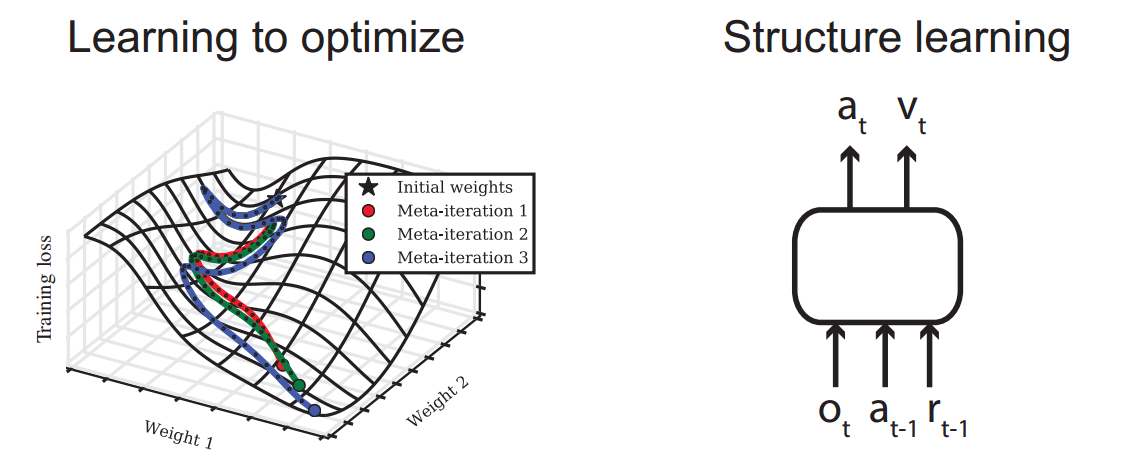
\includegraphics[scale=.19]{L2Optimize_StrLearning_Landsell.png}
  }}
  \caption{Types of learning-to-learn in AI. Learning-to-learn can be roughly divided into learning to optimize and structure learning.
  In AI, hyperparameter optimization is
  an example of learning to optimize (Maclaurin et al. 2015), while a recurrent neural network taking rewards, actions and observations
   can often be used to perform structure learning (Wang et al.)(Landsell et al.).}
        \label{figurelabel}
     \end{figure}


\subsection{Learning to Reinforcement Learn (metal-RL) and RL²}

A high level architecture consisting of a learner (performing on the task itself) and a meta-learner (adjusting the learner) is
inherent to most implementations of L2L (Landsell and Kording) and has been refined in various ways to create new L2L Systems, as will be
explained in the following section.

Wang et al. as well as Duan et al. introduced frameworks that can be thought of as generating an RL algorithm of their own and
provide agents, who are given a predesigned prior to efficiently learn any task $T \epsilon F$ (in the original papers denoted as 
a Markov Decision Process (MDP) $m \epsilon M$) from a family of interrelated fasks $F$(i.e. a set of MDPs $M$). 

In their attempt to design an algorithm, capable of performing well on a set $M$ of Markov Decision Processes (MDPs), Duan et al. implement a nested
system in which learning an RL algorithm is regarded as a reinforcement learning problem itself, hence the name RL²(Duan et al.). The agent performing 
on a randomly drawn separate MDP $m \epsilon M$ from the distribution $\rho_{M} : M \longrightarrow R_{+}$ is represented as a recurrent neural
network (RNN) which outputs the probability distribution over the tasks action-space $\pi$ (policy) based on a function $\phi (s,a,r,d)$ of 
the tuple (state, action, reward, termination flag) (Duan et al.). On a higher abstraction layer, this RNN is being 
optimized by an implementaion of Trust Region Policy Optimization (TRPO), a 
state-of-the-art DRL algorithm (Schulman et al., 2015) with several advantages regarding stability and hyperparameter dependance.\newline

\begin{figure}[thpb]
        \centering
        \framebox{\parbox{3in}{
        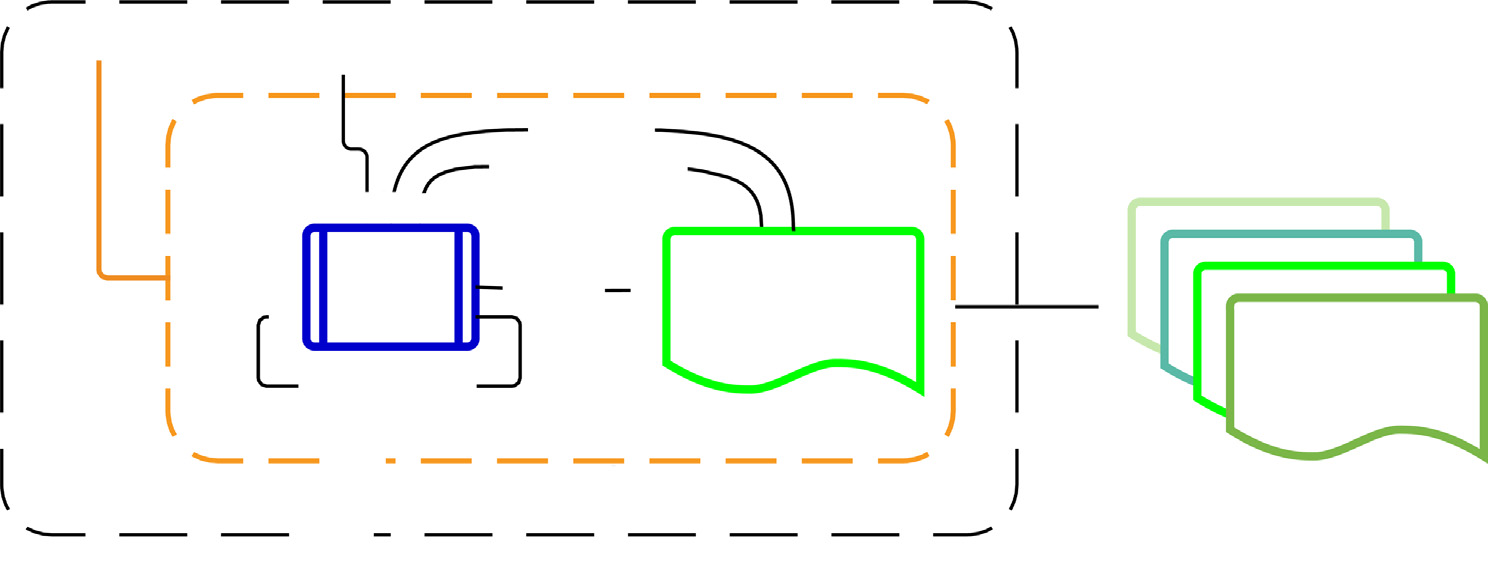
\includegraphics[scale=.185]{meta-RL_Botvinick.png}
  }}
  \caption{Schematic of Meta-reinforcement Learning, Illustrating the Inner and Outer Loops of Training. The
  outer loop trains the parameter weights $\theta$, which determine the inner-loop learner (’Agent’, instantiated by a recurrent
  neural network) that interacts with an environment for the duration of the episode. For every cycle of the outer loop, a new
  environment is sampled from a distribution of environments, which share some common structure (Botvinick et al.).}
        \label{figurelabel}
     \end{figure}

Wang et al. define a similiar setup in which a RL-algorithm is responsible for learning the weights of a nested RNN. Both, inner and outer loop 
in this framework draw their learning experience from the reward information generated by the actions of the RNN (Wang et al.), where 
the RNN holds information on the previously chosen action and the subsequent rewards. However the process of learning
in each of these loops is realized differently and results in specializations of different scopes. While the wrapping RL-algorithm used to 
optimize the weights of the RNN operates over the entire set of episodes, that is to say all MDPs $M$, learning of the nested RNN 
within a single task $m$ is based on the inner recurrent dynamics of the network. The policy outputs $\pi$ of this network can 
be viewed as an RL-algorithm on its own, resulting in the name meta-RL. For the implementation of this framework Wang et al. 
used a LSTM according to Hochreiter and Schmidhuber (Hochreiter and SChmidhuber, 1997) to account for the inner RNN, while both synchronous 
asynchronous advantage actor critics (A2C and A3C) (Mnih et al.) were employed to learn its parameters. The observation vectors of experiment environments
were either directly fed to the LSTM one-hot-encoded or passed through an additional deep encoder model (Wang et al.). 
Experiments on a series of bandit problem and two
MDP-centered problems with implementation architectures as described above showed, that meta-RL delivers 
competitive results compared to problem-specific algorithms (Thompson sampling, UCB, Gittins) while operating on a 
wider set of tasks. \newline

\begin{figure}[thpb]
        \centering
        \framebox{\parbox{3in}{
        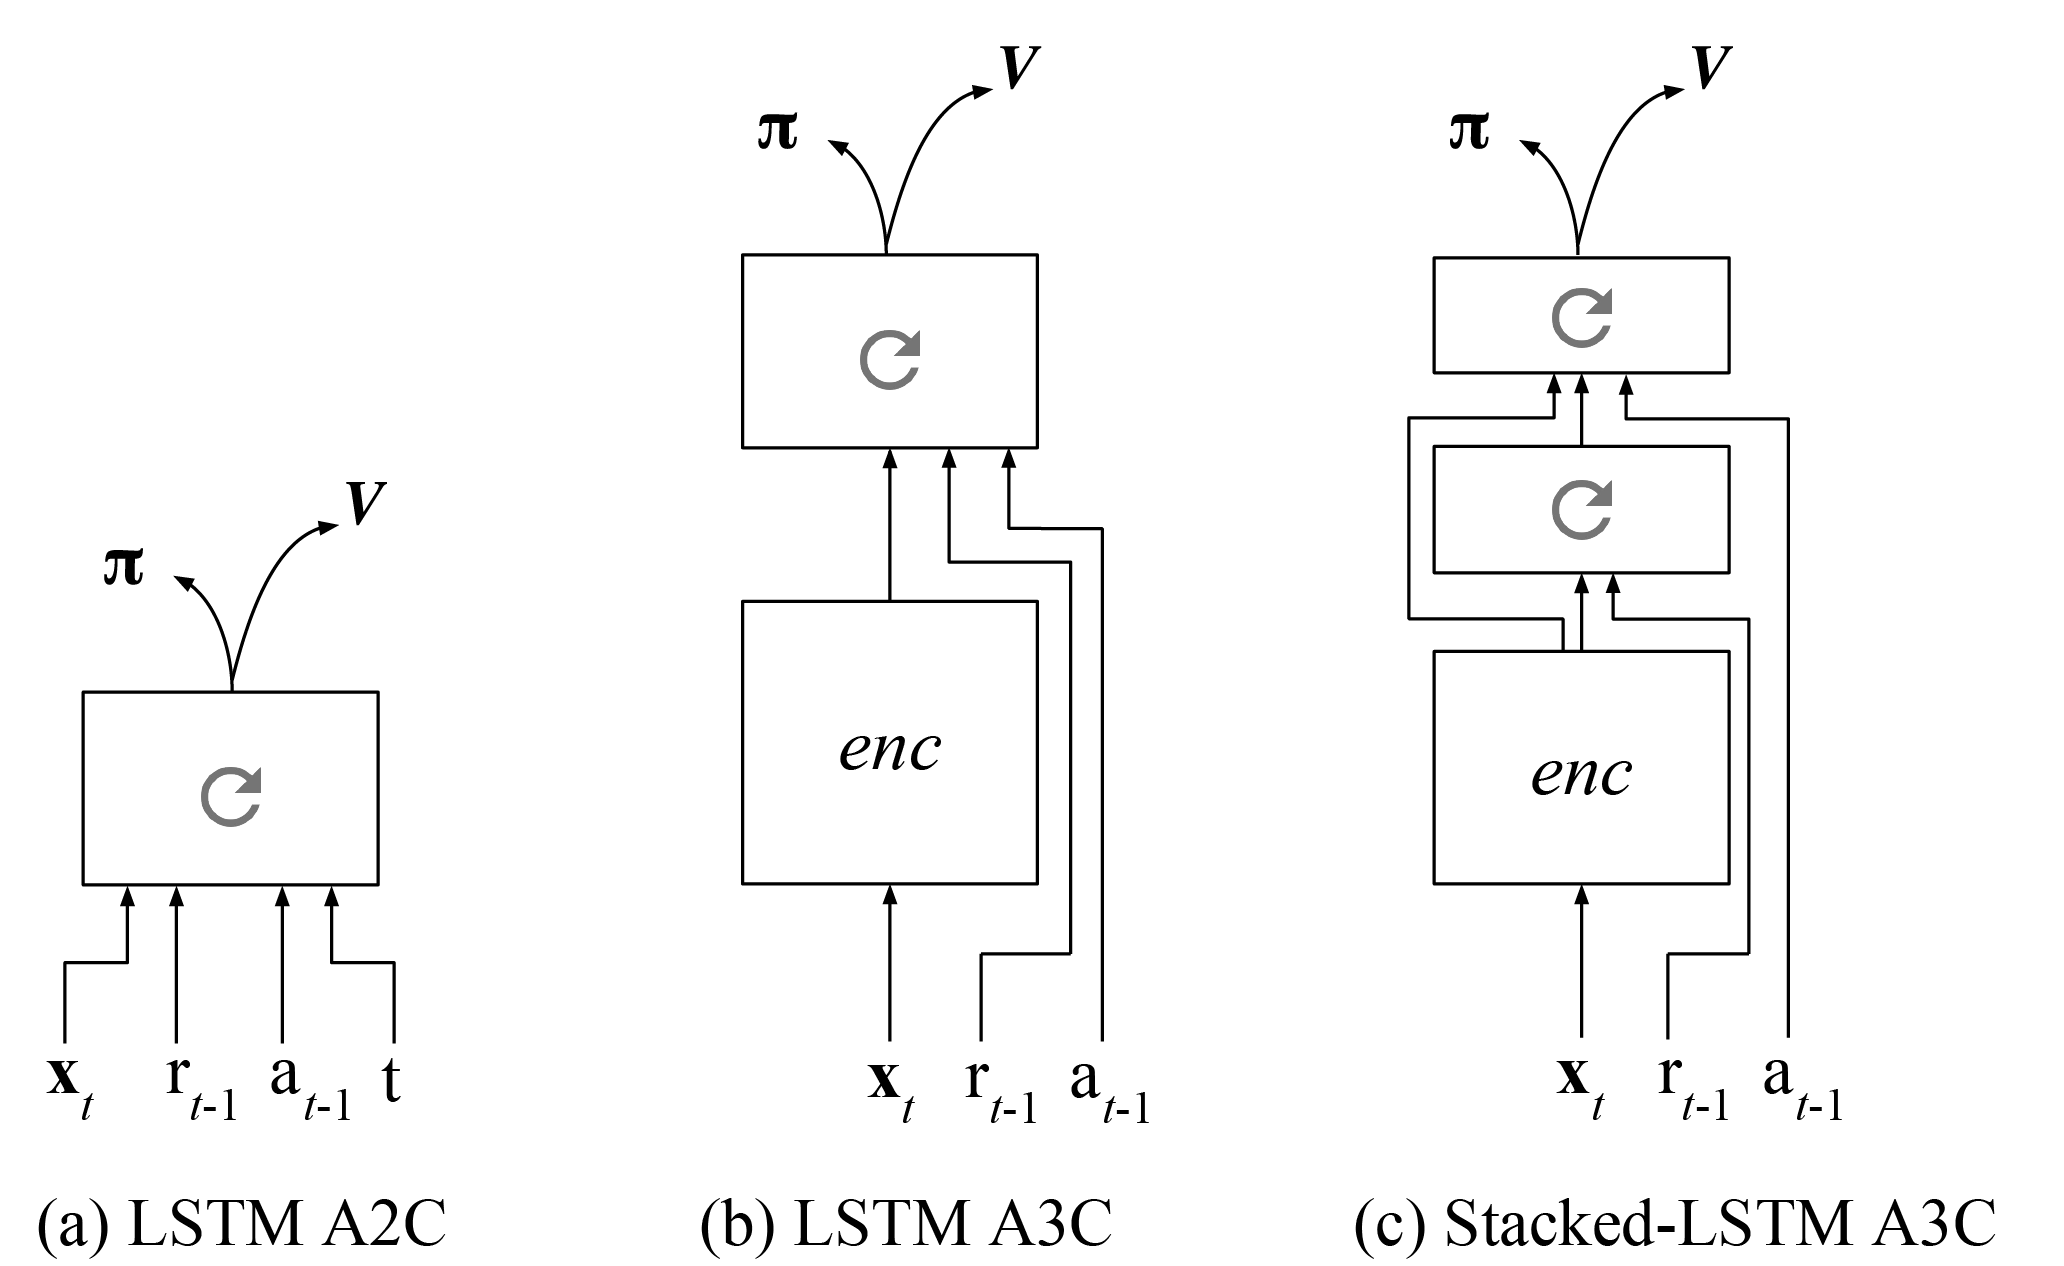
\includegraphics[scale=.14]{metaRL_arcs_Wang.png}
  }}
  \caption{Advantage actor-critic with recurrence. In all architectures, reward and last action are additional inputs
        to the LSTM. For non-bandit environments, observation is also fed into the LSTM either as a one-hot or passed
        through an encoder model [3-layer encoder: two convolutional layers (first layer: 16 8x8 filters applied with
        stride 4, second layer: 32 4x4 filters with stride 2) followed by a fully connected layer with 256 units and then a
        ReLU non-linearity. See for details Mirowski et al. (2016)]. For bandit experiments, current time step is also
        fed in as input. π = policy; v = value function. A3C is the distributed multi-threaded asynchronous version
        of the advantage actor-critic algorithm (Mnih et al., 2016); A2C is single threaded. (a) Architecture used in
        experiments 1-5. (b) Convolutional-LSTM architecture used in experiment 6. (c) Stacked LSTM architecture
        with convolutional encoder used in experiments 6 and 7 (Wang et al.)}
        \label{figurelabel}
     \end{figure}
  

A notable characteristic of both previously described setups is that the learning rate of the nested RNN is chosen lower compared 
to the outer optimization loop, consequently preventing
the agent from overfitting to a single task $m$, yet gathering knowledge from the entire MDP space $M$ (Botvinick et al.).\newline


more from :  \newline
Meta-SGD: Learning to Learn Quickly for Few-Shot Learning (Li et al.) \newline
Meta-learning in Reinforcement Learning (Schweighofer and Doya) \newline
Learning to Learn without Gradient Descent by Gradient Descent (Chen et al.)


\subsection{L2L in the Context of Spiking Neural Networks}

tbd \dots
Long short-term memory and Learning-to-learn in networks of spiking neurons (Bellec et al.)
Biologically inspired alternatives to backpropagation through time for learning in recurrent neural nets (Bellec et al.)
Embodied Neuromorphic Vision with Event-Driven Random Backpropagation (Kaiser et al.)

\subsection{Implications for Neuroscience and Psychology}
That is, having to learn their complete knowledge about the world from scratch, whereas the human brain has undergone a long history of evolutionary
development, adjusting its learning paradigms to the challenges it faces (Duan et al.). \newline

more from: \newline
Reinforcement Learning, Fast and Slow (Botvinick et al.) \newline
Biologically inspired alternatives to backpropagation through time for learning in recurrent neural nets (Bellec et al.) \newline
Towards learning-to-learn (Landsell and Kording) \newline

\section{APPLICATIONS OF L2L AND SNNS IN ROBOTICS}

Robotics has undergone many successful developments in the recent past with advances being pushed from 
numerous fields of engineering, including that of machine learning. Yet the design process is still a tedious and 
highly taylored one, requiring many domain experts. Many of the underlying algorithms in 
the control, motion planning and sensoric interpretation require suitable setups of the environment with little room
for variation. For example industrial manipulator robots can perform outstandingly when placed in a fixed production line, yet 
recognizing and grasping everyday objects in a kitchen or workshop poses a much higher challenge, as it requires the skill to 
make sense of broad environments with numerous imaginable tasks. Furthermore the dominating problems of applying RL in 
robotics can be summarized by the following problem classes (https://towardsdatascience.com/reinforcement-learning-for-real-world-robotics):

\begin{itemize}
        \item Sample efficiency
        \item Sim2Real
        \item Reward Specification
        \item Safety
\end{itemize}   

The previous sections revealed a high potential in L2L frameworks in terms of sample efficiency and generalization, thus constituting 
feasible answers to expensive data generation or overfitting to simulator-specific features. However this further implies a 
reflection on the scalability of said L2L approaches in order to evaluate their applicability in the often very
high-dimensional task spaces faced in robotics. \newline
Wang et al. examine meta-RL's ability to detect abstract task structures in large scale problems by adapting a well-known behavioural experiment 
described by Harlow (Harlow, 1949) to a visual fixation task. In Harlows experiment, monkeys were presented two unfamiliar objects, with one 
hiding a bowl filled with food and while the other holds an empty bowl. The monkeys were allowed to choose one of the objects and received the reward, if present. 
Despite switching the objects for new unkown objects in each episode, upon replaying several trials in several episodes of this game, the animals showed
a general understanding of the underlying structure of the problem. After beginning a new episode with new objects, the monkeys would, inevitably, take 
one random guess but managed to succeed in the following trials of the episode (Botvonick et al.). \newline

\subsection{Tasks in high-dimensional spaces}

Motion and path planning are fundamental problems in robotics, whether it be within a space of rich visual input, sensory data or
configuration/join-spaces. Similiar to the problem described by Harlow, the navigational task in the I-maze environment as described by 
Mirowski et al. and Jaderberg et al. requires a understanding of the general structure of the problem in order to learn sample-efficiently 
on the specific task. In this case the same maze spawns a goal location on random position within the maze where the agent has to learn
a motion path to the goal in as few trials as possible. The results of Wang et al. show, that an architecture of stacked LSTM is able to 
solve the task after having conducted one exploration run (finishing the episode in ~100 timesteps) notably faster (~30 timesteps) within few
explotation runs. The reference baseline, a feedforward architecture A3C learner, is not able to solve the problem at all. 
 
\begin{figure}[thpb]
        \centering
        \framebox{\parbox{3in}{
        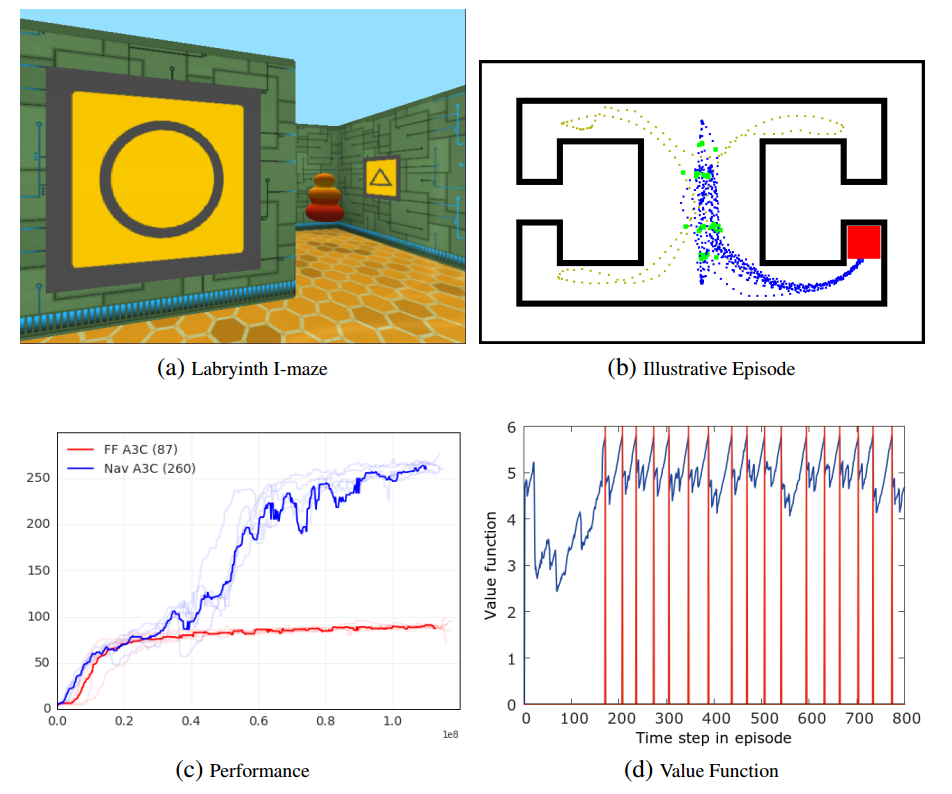
\includegraphics[scale=.23]{Maze_wang.png}
  }}
  \caption{a) view of I-maze showing goal object in one of the 4 alcoves b) following initial exploration
  (light trajectories), agent repeatedly goes to goal (blue trajectories) c) Performance of stacked LSTM (termed
  “Nav A3C”) and feedforward (“FF A3C”) architectures, per episode (goal = 10 points) averaged across top 5
  hyperparameters. e) following initial goal discovery (goal hits marked in red), value function occurs well in
  advance of the agent seeing the goal which is hidden in an alcove.
  }
        \label{figurelabel}
     \end{figure}

Duan et al. take a similiar approach in their evaluation of the feasbility of RL² in high-dimensional state spaces. Again a randomly generated 
maze with a randomly placed target is chosen as the problem to solve for the agent. During one test run, the agent is given a number 
of episodes during which the maze structure and target position remain fixed. In contrast to an earlier approach to this RL-Task shown by Oh et al. 
RL² bases its actions within a more granular action space (Duan et al.). The environments sparse reward payout design (+1 for target, 
-0.001 for wall hits, -0.04 per time frame) poses additional challenges to the agents learning and requires well-devloped exploration strategies 
in the first episode in order to gain information on the problems ground structure. Cross-validation with a small and a larger version of the 
maze environment show a significant reduction in solving trajectory lengths between the first to episodes and indicate, that the RL² algorithm 
managed to utilize previoulsy gained information to come to good solutions more quickly. However the shown results are not yet optimal
as the agent still forgets, though rarely, initially explored target positions and explores further paths in the second episode. Duan et al. 
indicate that further imporvements might come with improved RL-algorithms as the outer-loop optimizer.

\begin{figure}[thpb]
        \centering
        \framebox{\parbox{3in}{
        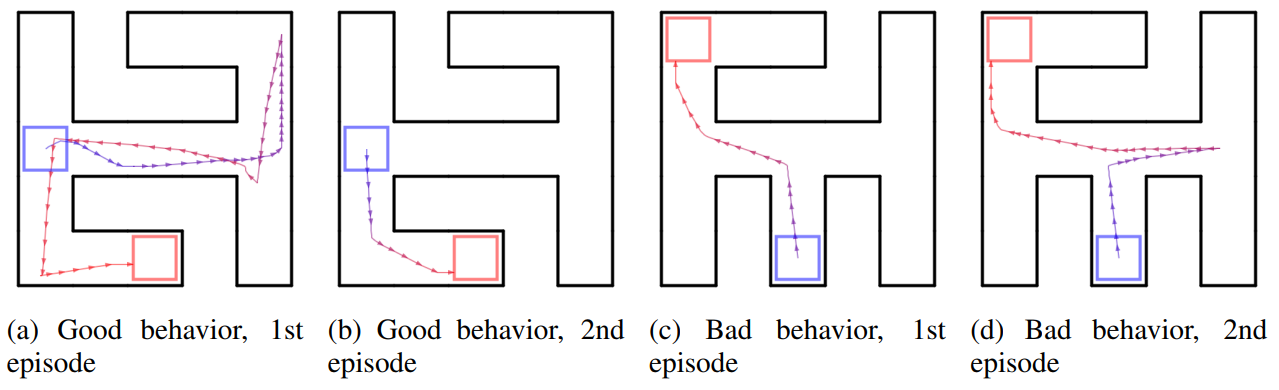
\includegraphics[scale=.23]{duan_maze.png}
  }}
  \caption{Visualization of the agent’s behavior. In each scenario, the agent starts at the center of the
  blue block, and the goal is to reach anywhere in the red block.  
  }
        \label{figurelabel}
     \end{figure}

more from :  \newline
Meta-SGD: Learning to Learn Quickly for Few-Shot Learning (Li et al.) \newline
Meta-learning in Reinforcement Learning (Schweighofer and Doya) \newline
Learning to Learn without Gradient Descent by Gradient Descent (Chen et al.)

\subsection{Speed Improvement and Few-Shot Learning}

\section{CONCLUSION AND CHALLENGES}

\addtolength{\textheight}{-12cm}   % This command serves to balance the column lengths
                                  % on the last page of the document manually. It shortens
                                  % the textheight of the last page by a suitable amount.
                                  % This command does not take effect until the next page
                                  % so it should come on the page before the last. Make
                                  % sure that you do not shorten the textheight too much.

%%%%%%%%%%%%%%%%%%%%%%%%%%%%%%%%%%%%%%%%%%%%%%%%%%%%%%%%%%%%%%%%%%%%%%%%%%%%%%%%



%%%%%%%%%%%%%%%%%%%%%%%%%%%%%%%%%%%%%%%%%%%%%%%%%%%%%%%%%%%%%%%%%%%%%%%%%%%%%%%%



%%%%%%%%%%%%%%%%%%%%%%%%%%%%%%%%%%%%%%%%%%%%%%%%%%%%%%%%%%%%%%%%%%%%%%%%%%%%%%%%
\section*{APPENDIX}

Appendixes should appear before the acknowledgment.

%%%%%%%%%%%%%%%%%%%%%%%%%%%%%%%%%%%%%%%%%%%%%%%%%%%%%%%%%%%%%%%%%%%%%%%%%%%%%%%%

\begin{thebibliography}{99}

\bibitem{c1}




\end{thebibliography}




\end{document}
